%     LINEAR ALGEBRA
%----------------------------------------------------------------------------------------------------
\lstset{ %
  language=Matlab,                     % choose the language of the code
  basicstyle=\footnotesize,            % the size of the fonts that are used for the code
  backgroundcolor=\color{white},       % choose the background color. You must add \usepackage{color}
  commentstyle=\color{help}\textit,
  keywordstyle=\color{keyword}\textbf,
  breaklines=true,                     % sets automatic line breaking
  breakatwhitespace=true,              % sets if automatic breaks should only happen at whitespace
  showspaces=false,                    % show spaces adding particular underscores
  showstringspaces=true,               % underline spaces within strings
  showtabs=true,                       % show tabs within strings adding particular underscores
  frame=none,	                       % adds a frame around the code - none, single
  tabsize=8,                           % sets default tabsize to 8 spaces
  captionpos=b,                        % sets the caption-position to bottom
  numbers=left,                        % where to put the line-numbers -none, left, right
  numberstyle=\footnotesize,           % the size of the fonts that are used for the line-numbers
  stepnumber=1,                        % the step between two line-numbers. If it's 1 each line
                                       % will be numbered
  xleftmargin=3em,                     % adjust left margin
}
%----------------------------------------------------------------------------------------------------
% Setting path to image 
\graphicspath{{../src/LA/img/}}  
%--------------------Introduction to linear algebra--------------------------------------------------
  %     Basis of Linear Algebra:
% ============================================================================================================
% In linear algebra, a basis is a set of linearly independent vectors that, in a
% linear combination, can represent every vector in a given vector space or free
% module, or, more simply put, which define a "coordinate system".[1] In more
% general terms, a basis is a linearly independent spanning set. 
% ------------------------------------------------------------------------------------------------------------
\chapter{Základy lineární algebry}
\minitoc
\newpage
  \section{Matice}
    \begin{definition}\label{def_matice}
      Nechť $m$,$n$ jsou přirozená čísla. Jestliže každé uspořádané dvojici $(m,n)$. Jestliže každé
      uspořádané dvojici $(m,n)\in \{1,2,\ldots,m\}\times \{1,2,\ldots,m\}$ přiřadíme prvek
      $a_{i,j}\in\mathcal{R}$ obdržíme reálnou \href{http://cs.wikipedia.org/wiki/Matice}{matici} typu 
      $(m,n)$ nad $\mathcal{R}$. Čísla jsou indexy, $i$ je řádkový a $j$ je sloupcový index.
      
      Matici zapisujeme jako
      \begin{equation}\label{matice_zapis}
        A = \left(a_{ij}\right) =\left(
          \begin{array}{ccc}
            a_{11} & \ldots & a_{1n} \\
            \vdots & \ddots & \vdots \\
            a_{m1} & \ldots & a_{nn}
          \end{array}
        \right)
      \end{equation}
      která má právě $ mn $ prvků $ \left(a_{ij}\right) $ uspořádaných do $ m $ řádků a $ n $ sloupců. 
      Stručně píšeme $ A = \left(a_{ij}\right) $
    \end{definition}
  
    \begin{example}
      Matice
      \begin{displaymath}
          \left(\begin{array}{rrrr}1&2&3&4\\4&3&2&1\\-1&-1&-1&-1\\-2&-1&0&1\end{array}\right)
      \end{displaymath}
      je čtvercová matice velikosti 4x4. Prvek matice $ a_{23} $ je 2.
    \end{example}  
    
    \subsection{Maticová algebra}
      \begin{definition} 
        Součinem matice $A \in \mathcal{R}_{m,n}$ a matice $B \in \mathcal{R}_{n,p}$, v uvedeném
        pořadí, je matice $C \in \mathcal{R}_{m;p}$ pro kterou platí:
        \begin{equation}
           C = AB; C = (cij); cij = \sum_n^{k=1}{a_{ik}b_{kj}}; i = 1,\ldots,m; j = 1,\ldots,p.
        \end{equation} 
      \end{definition}  
      Součin matic $A$ a $B$ je definován právě tehdy, když počet sloupců matice $A$ je roven počtu 
      řádků matice $B$. Obrázek \ref{LA:fig_matrix_multipl_step1} demonstruje jakým způsobem se dostane 
      prvek, který je ve výsledné matici třeba ve druhém řádku a druhém sloupci, násobením druhého řádku levé 
      matice s druhým sloupcem pravé ze zadaných matic. Stejným způsobem získáme hodnotu prvku $c_{ij}$ (viz 
      \ref{LA:fig_matrix_multipl_step2}).
      %----------------------------------
        % image: LA_matrix_multiplication.tex label: 
        % \label{LA:fig_matrix_multipl_step1} \label{LA:fig_matrix_multipl_step2}
        % \documentclass{article}
%  \usepackage{tikz}                      % TikZ and PGF picture 
%      \usetikzlibrary{intersections}
%      \usetikzlibrary{calc}
%      \usetikzlibrary{positioning}  
%      \usetikzlibrary{decorations.markings}
%      \usetikzlibrary{decorations.pathmorphing}   
%      \usetikzlibrary{shapes}
%      \usetikzlibrary{matrix,chains,scopes}
%      \usetikzlibrary{arrows,fit}
%       \usepackage{amsmath, amsthm, amssymb, amsfonts, amsbsy}  
% \usepackage{xltxtra,unicode-math} 
%      \setmainfont[Mapping=tex-text,Numbers={OldStyle,Proportional}]{Calibri} % Linux Libertine , Calibri, Constantia
%      \setsansfont[Mapping=tex-text,Numbers={OldStyle,Proportional}]{Candara}
%      \setmonofont[Numbers=OldStyle]{Consolas}  
%      \setmathfont{Cambria Math}    % (Microsoft),
%  \usepackage{wrapfig}                   % Floats, Figures and Captions  
%  \usepackage{subfigure}                 % Multipart figures
%  \usepackage{tikz}                      % TikZ and PGF picture 
%       \usetikzlibrary{intersections}
%       \usetikzlibrary{calc}
%       \usetikzlibrary{positioning}     
%  
% \begin{document}
\newcommand{\myunit}{0.9 cm}
  \tikzset{
          node  style    sp/.style={draw,circle,minimum size=\myunit},
          node  style    ge/.style={circle,minimum size=\myunit}, 
          arrow style   mul/.style={draw,sloped,midway,fill=white}, 
          arrow style  plus/.style={midway,sloped,fill=white},
      }
      
      \begin{figure}
        \centering
        \begin{tikzpicture}[>=latex, scale=0.8, every node/.style={scale=0.8}]
          % les matrices
          \matrix (A) [matrix of math nodes,%
                       nodes = {node style ge},%
                       left delimiter  = (,%
                       right delimiter = )] at (0,0)
          {%
            a_{11} & a_{12} & \ldots & a_{1p}  \\
            \node[node style sp] {a_{21}};%
                   & \node[node style sp] {a_{22}};%
                            & \ldots%
                                     & \node[node style sp] {a_{2p}}; \\
            \vdots & \vdots & \ddots & \vdots  \\
            a_{n1} & a_{n2} & \ldots & a_{np}  \\
          };
          \node [draw,below=10pt] at (A.south) 
              { $A$ : \textcolor{red}{$n$ rows} $p$ columns};
          
          \matrix (B) [matrix of math nodes,%
                       nodes = {node style ge},%
                       left delimiter  = (,%
                       right delimiter =)] at (6*\myunit,6*\myunit)
          {%
            b_{11} & \node[node style sp] {b_{12}};%
                            & \ldots & b_{1q}  \\
            b_{21} & \node[node style sp] {b_{22}};%
                            & \ldots & b_{2q}  \\
            \vdots & \vdots & \ddots & \vdots  \\
            b_{p1} & \node[node style sp] {b_{p2}};%
                            & \ldots & b_{pq}  \\
          };
          \node [draw,above=10pt] at (B.north) 
              { $B$ : $p$ rows \textcolor{red}{$q$ columns}};
          % matrice resultat
          \matrix (C) [matrix of math nodes,%
                       nodes = {node style ge},%
                       left delimiter  = (,%
                       right delimiter = )] at (6*\myunit,0)
          {%
            c_{11} & c_{12} & \ldots & c_{1q} \\
            c_{21} & \node[node style sp,red] {c_{22}};%
                            & \ldots & c_{2q} \\
            \vdots & \vdots & \ddots & \vdots \\
            c_{n1} & c_{n2} & \ldots & c_{nq} \\
          };
          % les fleches
          \draw[blue] (A-2-1.north) -- (C-2-2.north);
          \draw[blue] (A-2-1.south) -- (C-2-2.south);
          \draw[blue] (B-1-2.west)  -- (C-2-2.west);
          \draw[blue] (B-1-2.east)  -- (C-2-2.east);
          \draw[<->,red](A-2-1) to[in=180,out=90]
            node[arrow style mul] (x) {$a_{21}\times b_{12}$} (B-1-2);
          \draw[<->,red](A-2-2) to[in=180,out=90]
            node[arrow style mul] (y) {$a_{22}\times b_{22}$} (B-2-2);
          \draw[<->,red](A-2-4) to[in=180,out=90]
            node[arrow style mul] (z) {$a_{2p}\times b_{p2}$} (B-4-2);
          \draw[red,->] (x) to node[arrow style plus] {$+$} (y)%
                            to node[arrow style plus] {$+\raisebox{.5ex}{\ldots}+$} (z)%
                            to (C-2-2.north west);   
          \node [draw,below=10pt] at (C.south) 
              {$ C=A\times B$ : \textcolor{red}{$n$ rows}  \textcolor{red}{$q$ columns}};  
        \end{tikzpicture}
        \caption[Násobení matic]{Násobení matic - 1. krok}\label{LA:fig_matrix_multipl_step1}
      \end{figure}
      
      \begin{figure}
        \centering
        \begin{tikzpicture}[>=latex, scale=0.8, every node/.style={scale=0.8}]
          % unit
          % defintion of matrices
          \matrix (A) [matrix of math nodes,%
                       nodes = {node style ge},%
                       left delimiter  = (,%
                       right delimiter = )] at (0,0)
          {%
            a_{11} &\ldots  & a_{1k} & \ldots & a_{1p}  \\
            \vdots & \ddots & \vdots & \vdots & \vdots \\
            \node[node style sp] {a_{i1}};& \ldots %
                   & \node[node style sp] {a_{ik}};%
                            & \ldots%
                                     & \node[node style sp] {a_{ip}}; \\
            \vdots & \vdots& \vdots & \ddots & \vdots  \\
            a_{n1}& \ldots & a_{nk} & \ldots & a_{np}  \\
          };
          \node [draw,below] at (A.south) { $A$ : \textcolor{red}{$n$ rows} $p$ columns};
          \matrix (B) [matrix of math nodes,%
                       nodes = {node style ge},%
                       left delimiter  = (,%
                       right delimiter =)] at (7*\myunit,7*\myunit)
          {%
            b_{11} &  \ldots& \node[node style sp] {b_{1j}};%
                            & \ldots & b_{1q}  \\
            \vdots& \ddots & \vdots & \vdots & \vdots \\
            b_{k1} &  \ldots& \node[node style sp] {b_{kj}};%
                            & \ldots & b_{kq}  \\
            \vdots& \vdots & \vdots & \ddots & \vdots \\
            b_{p1} &  \ldots& \node[node style sp] {b_{pj}};%
                            & \ldots & b_{pq}  \\
          };
          \node [draw,above] at (B.north) { $B$ : $p$ rows \textcolor{red}{$q$ columns}};
          % matrice resultat
          \matrix (C) [matrix of math nodes,%
                       nodes = {node style ge},%
                       left delimiter  = (,%
                       right delimiter = )] at (7*\myunit,0)
          {%
            c_{11} & \ldots& c_{1j} & \ldots & c_{1q} \\
            \vdots& \ddots & \vdots & \vdots & \vdots \\
              c_{i1}& \ldots & \node[node style sp,red] {c_{ij}};%
                            & \ldots & c_{iq} \\
            \vdots& \vdots & \vdots & \ddots & \vdots \\
            c_{n1}& \ldots & c_{nk} & \ldots & c_{nq} \\
          };
          \node [draw,below] at (C.south) 
              {$ C=A\times B$ : \textcolor{red}{$n$ rows}  \textcolor{red}{$q$ columns}};
          % arrows
          \draw[blue] (A-3-1.north) -- (C-3-3.north);
          \draw[blue] (A-3-1.south) -- (C-3-3.south);
          \draw[blue] (B-1-3.west)  -- (C-3-3.west);
          \draw[blue] (B-1-3.east)  -- (C-3-3.east);
          \draw[<->,red](A-3-1) to[in=180,out=90] 
              node[arrow style mul] (x) {$a_{i1}\times b_{1j}$} (B-1-3);
          \draw[<->,red](A-3-3) to[in=180,out=90] 
              node[arrow style mul] (y) {$a_{ik}\times b_{kj}$}(B-3-3);
          \draw[<->,red](A-3-5) to[in=180,out=90] 
              node[arrow style mul] (z) {$a_{ip}\times b_{pj}$}(B-5-3);
          \draw[red,->] (x) to node[arrow style plus] {$+\raisebox{.5ex}{\ldots}+$} (y)%
                            to node[arrow style plus] {$+\raisebox{.5ex}{\ldots}+$} (z);
                            %
                            % to (C-3-3.north west);
          \draw[->,red,decorate,decoration=zigzag] (z) -- (C-3-3.north west);
        \end{tikzpicture}
        \caption[Násobení matic]{násobení matic - 2. krok}\label{LA:fig_matrix_multipl_step2}
      \end{figure}
% \end{document}      
      %---------------------------------- 
  
    %--------------------------------------------------------------------------------------------------
    \subsection{Označení prvků matice}
      Prvky matice jsou označeny indexy udávajícími \textbf{řádek} a \textbf{sloupec}, v nichž se prvek 
      nalézá. Prvek v i-tém řádku a j-tém sloupci matice $A$ se obvykle značí $a_{ij}$. Potom i-tý řádek 
      matice  obsahuje vodorovnou n-tici prvků $(a_{i1},a_{i2},\ldots,a_{in} )$, kde $i =  1,2,\ldots,m$ a 
      j-tý sloupec matice obsahuje svislou matici čísel $(a_{1j},a_{2j},\ldots,a_{mj})$, kde $j =       
      1,2,\ldots,n$.
  
      V tabulce \ref{LA:tab_basic_matrix} jsou uvedeny nejčastější typy matic, které se v algebře často 
      vyskytují. Jsou to například matice řádkové, sloupcové, diagonální\footnote{Prvky $a_{ii}$ kde 
      $i=1,2,\ldots,\min(m,n)$ tvoří hlavní diagonálu. Matice $\mathbf{D}$ je typu $(m,m)$, obecně může mít 
      diagonální matice buď ještě další sloupce, v nichž budou samé nuly, anebo další řádky, v nichž budou 
      opět samé nuly.}, jednotkové\footnote{ Jestliže $m = n$, pak mluvíme o čtvercové matici řádu $m$.}, 
      nulové, transponované a symetrické.
  
      \begin{table}[!ht]
          \centering
            \begin{tabular}{|l|c c l|}\hline
              \textbf{Matice} & \multicolumn{3}{|c|}{\textbf{Zápis}} \\ \hline
              \ttfamily řádková & $ \mathbf{A} $ & $ = $ & $(a_1,a_2,\ldots,a_n )$\\
              \ttfamily sloupcová & $ \mathbf{B} $ & $ = $ & $\left(
                \begin{array}{c}
                  a_1     \\
                  a_2     \\
                  \vdots  \\
                  a_n
                \end{array}
              \right) $\\
              \multirow{2}{*}{\ttfamily diagonální} & \multicolumn{3}{|c|}{ $ a_{ij}= 0 \forall i
              \neq j$}\\
               & $ \mathbf{C}$ & $ = $ & $ \left(
                \begin{array}{cccc}
                  a_{11} &    0   & \ldots &   0    \\
                     0   & a_{22} & \ldots &   0    \\
                  \vdots & \vdots & \ddots & \vdots \\
                     0   &   0    & \ldots & a_{mm}
                \end{array}\right) $\\
              \ttfamily jednotková & $ \mathbf{I}$ & $ = $ & $\left(
                \begin{array}{cccc}
                     1    &    0   & \ldots &   0    \\
                     0    &    1   & \ldots &   0    \\
                   \vdots & \vdots & \ddots & \vdots \\
                      0   &   0    & \ldots & 1
                \end{array}\right) $\\
              \ttfamily nulová & $ \mathbf{0}$ & $ = $ & $ (a_{ij}),\quad a_{ij} = 0 \forall i, j $\\
              \ttfamily transponovaná & $ \mathbf{D^T} $ & $ = $ & $ \left(
                \begin{array}{cccc}
                  a_{11} & a_{21} & \ldots &  a_{m1}\\
                  a_{12} & a_{22} & \ldots &  a_{m2}\\
                  \vdots & \vdots & \ddots & \vdots \\
                  a_{1n} & a_{2n} & \ldots & a_{mn}
                \end{array}\right) $\\
              \ttfamily symetrická & $\mathbf{S}$ & $ = $ & $ (a_{ij}),\quad a_{ij}= a_{ji}\forall
              i,j $\\ \hline
            \end{tabular}
          \caption{Speciální typy matic}\label{LA:tab_basic_matrix}
      \end{table}
    
    
      Matice téhož typu $\left(m,n\right)$ nad $\Re$ budeme značit $\Re_{m,n}$.
      \begin{definition}\label{rovnost_matic}
       (Rovnost matic):  Matice $\mathbf{A} = \left(a_{ij}\right)$ je rovna matici $\mathbf{B}=
       \left(b_{kl}\right)$, jsou-li matice stejného typu a stejnolehlé prvky se sobě
       \textbf{rovnají}, tj. $\mathbf{A} \in \Re_{m,n}, \mathbf{B}\in\Re_{m,n}, a_{ij} = b_{ij}, 
       \forall i\in\lbrace1,2,\ldots,m\rbrace, \forall j\in\lbrace1,2,\ldots,n\rbrace$.
      \end{definition}    
   
  %===============================Kapitola: Determinanty======================================================
  \section{Determinanty}
    Abychom mohli nadefinovat determinant, budeme muset vědět, jak vypočítat permutaci entice, respektive 
    znaménko permutace.
    \subsection{Permutace}
      \begin{definition}\label{permutace}
        Nechť $\mathbf{M}$ je libovolná konečná množina. Permutací množiny M nazýváme zobrazení $\pi$
        množiny $\mathbf{M}$ na sebe.
      \end{definition}
      
      \begin{example}%(Damlová  Nagy, 1985, str. 34)
        Permutace $\pi$ množiny $\mathbf{M}= \lbrace a,b,c,d\rbrace$ je např. zobrazení 
        $\pi$, definované předpisem:
        \begin{equation}\label{permutace_zadani}
          \pi\left(a\right) = c, \pi\left(b\right) = d, \pi\left(c\right) = b, \pi\left(d\right) = a,
        \end{equation}
        Místo tohoto zápisu se však používá přehlednější zápis ve tvaru matice typu
        $\left(2,4\right)$:
        \begin{equation}\label{LA:eq_perm_exam}
          \left(
            \begin{array}{cccc}
            a & b & c & d \\
            c & d & b & a
            \end{array}
          \right)
        \end{equation}
        kde v prvním řádku jsou vypsány všechny prvky množiny $\mathbf{M}$ (v libovolném pořadí) a ve druhém 
        řádku je pod každým prvkem zapsán jeho obraz v permutaci. Tutéž permutaci však můžeme zapsat ve tvaru 
        matice několika různými způsoby. Například mohou být zapsány takto:
        \begin{equation}
          \left(
            \begin{array}{cccc}
            b & a & c & d \\
            d & c & b & a
            \end{array}
          \right),\quad
          \left(
            \begin{array}{cccc}
            d & c & b & a \\
            a & b & d & c
            \end{array}
            \right),\quad
          \left(
            \begin{array}{cccc}
            d & c & a & b \\
            a & b & c & d
            \end{array}
          \right),\quad apod.
        \end{equation}
      \end{example}
      Zřejmě všechny čtyři uvedené zápisy permutace rov. \ref{LA:eq_perm_exam} ve tvaru matice se liší 
      navzájem pouze pořadím sloupců. Aby bylo možné zapsat každou permutaci množiny $\mathbf{M}$ ve tvaru 
      rov. \ref{LA:eq_perm_exam} jediným způsobem, je nutné zvolit pevné pořadí prvků množiny $\mathbf{M}$  a 
      v zápisu permutace uvádět prvky matice $\mathbf{M}$  v prvním řádku v tomto pořadí. Avšak známe-li toto 
      pořadí prvků množiny $\mathbf{M}$, je pak obvykle zbytečné jej v zápisu permutace uvádět, ale stačí 
      uvést pouze pořadí obrazů, tj. druhý řádek. Zvolíme-li např. v naší množině $\mathbf{M}$pevné pořadí 
      prvků $\lbrace a,b,c,d\rbrace$,pak permutaci rov. \ref{permutace_zadani} zapíšeme jako uspořádanou 
      čtveřici $\lbrace c,d,b,a\rbrace$.
  
      \begin{definition}\label{def_permutace_ntice}
        Když vytváříme uspořádanou n-tici navzájem různých prvků n-prv\-ko\-vé množiny $\mathbf{M}$,
        přiřazujeme každému prvku množiny $\mathbf{M}$ právě jedno přirozené číslo, index příslušného
        prvku, z množiny prvních $n$ přirozených čísel.
        \begin{equation}\label{permutace_ntice}
          \pi = \lbrace 1, 2, 3, \ldots, n\rbrace
        \end{equation}
      \end{definition}
  
      Proto každé permutaci uspořádané n-tice prvků množiny $\mathbf{M}$ odpovídá jednoznačně permutace 
      příslušných indexů tj. permutace množiny \ref{permutace_ntice} z definice \ref{def_permutace_ntice}. 
      Stačí se tedy omezit při vyšetřování permutací n-prvkové množin na vyšetřování permutací množiny 
      \ref{permutace_ntice}. Permutace $\pi$ množiny \ref{permutace_ntice} budeme zapisovat jako uspořádané 
      n-tice $$\left(\pi(1), \pi(2) ,\ldots, \pi(n)\right)$$, kde $\pi(i)$ je číslo z množiny
      \ref{permutace_ntice}, které permutace $\pi$ přiřazuje číslu $i$.
      \begin{example}\label{ex_celk_pocet_permutaci}\textbf{Spočítejme celkový počet permutací
        množiny}. V kaž\-dé uspořádané n-tici může být na prvním místě kterákoli z $n$ cifer, na
        druhém místě kterákoli ze zbývajících $n-1$ cifer (kromě té, která je na prvním místě), na
        třetím místě každá ze zbývajících $n-2$ cifer atd. Je tedy celkový počet všech permutací
        n-prvkové množiny $n(n-1)(n-2)\cdot \ldots \cdot2\cdot1$.
        Toto číslo se zapisuje pomocí symbolu $n!$ (čti \textbf{n-faktoriál}).
      \end{example}
      \begin{definition}\label{def_inv_perm}\textbf{Inverze v permutaci}:
        Inverzí v permutaci $\left(i_1,i_2,…,i_n \right)$ rozumíme každý výskyt takové dvojice čísel,
        že větší stojí před menším, tj. vlevo od něj.
      \end{definition}  
   
  %=============================Kapitola: Vlastní čísla a vlastní vektory ===========================
  \section{Vlastní čísla a vlastní vektory}
    \subsection{Motivace} 
      \textbf{Poznámka}: Je-li $\mathcal{A} : \mathcal{V} \rightarrow \mathcal{V}$ lineární zobrazení z 
      prostoru $\mathcal{V}$ do prostoru $\mathcal{V}$ (nikdy se takové zobrazení nazývá lineárním       
      operátorem), pak je přirozeným požadavkem najít takovou bázi prostoru $\mathcal{V}$, že je matice 
      zobrazení $\mathbf{A}$ v této bázi co nejjednodušší, např. má následující strukturu
       \begin{equation*}
          \mathbf{A}=
            \left(\begin{array}{ccccc}
              \boxed{A_1}       &             &       &       & 0   \\
                  & \boxed{A_2} &             &       &             \\
                  &             & \boxed{A_3} &       &             \\
                  &             &             &\ddots &             \\
               0  &             &             &       & \boxed{A_k}
             \end{array}
            \right),
       \end{equation*}
      kde $A_k$ jsou čtvercové matice malého řádu (nejlépe 1 nebo 2) a ostatní prvky matice jsou nulové. 
      Problém najít bázi, aby v ní matice zobrazení měla diagonální tvar (kde $A_k$ jsou skaláry), vede k 
      pojmu vlastní číslo a vlastní vektor matice.
      \begin{definition} Nechť $\mathbf{A}\in \mathcal{C}^{n,n}$(matice je čtvercová řádu $n$).     
        $$A = \left(a_{ij}\right) =
        \left(
          \begin{array}{cccc}
            a_{11} & a_{12} & \ldots & a_{1n} \\
            a_{21} & a_{22} & \ldots & a_{2n} \\
            \vdots & \vdots & \ddots & \vdots \\
            a_{n1} & a_{n2} & \ldots & a_{nn}
          \end{array}
        \right)$$
        Jestliže platí
        \begin{equation}\label{eq:vl_number}
          \mathbf{Au} = \lambda\mathbf{u}
        \end{equation}
        pro jisté komplexní číslo $\lambda\in\mathcal{C}$  a jistý nenulový vektor $x\in\mathcal{C}^n, 
        \mathbf{u}\neq\Theta$, potom číslo $\lambda$ nazýváme \textbf{vlastním číslem} matice $\mathbf{A}$ a 
        vektor $\mathbf{u}$ \textbf{vlastním vektorem} příslušným k tomuto vlastnímu číslu. Množinu všech 
        vlastních čísel nazýváme \textbf{spektrem matice} $\mathbf{A}$.Pokud rov. \ref{eq:vl_number} 
        rozepíšeme, dostaneme
        \begin{equation}
          \left(
            \begin{array}{cccc}
              a_{11} & a_{12} & \ldots & a_{1n} \\
              a_{21} & a_{22} & \ldots & a_{2n} \\
              \vdots & \vdots & \ddots & \vdots \\
              a_{n1} & a_{n2} & \ldots & a_{nn}
            \end{array}
        \right)\cdot
        \left(
          \begin{array}{c}
            u_{1} \\  u_{2} \\ \vdots \\  u_{n} \\
          \end{array}
        \right)=\lambda\cdot
        \left(
          \begin{array}{c}
            u_{1} \\ u_{2} \\ \vdots \\ u_{n} \\
          \end{array}
        \right)
        \end{equation}
        můžeme ji rovněž psát ve tvaru
        \begin{equation}\label{def_vv_homogenni}
          \left(
            \begin{array}{cccc}
              a_{11} -\lambda & a_{12}           & \ldots & a_{1n} \\
              a_{21}          & a_{22} -\lambda  & \ldots & a_{2n} \\
              \vdots          & \vdots           & \ddots & \vdots \\
              a_{n1}          & a_{n2}           & \ldots & a_{nn}-\lambda
            \end{array}
          \right)\cdot\left(
          \begin{array}{c}
            u_{1} \\ u_{2} \\ \vdots \\ u_{n} \\
          \end{array}
          \right)=
          \left(
            \begin{array}{c}
              0 \\ 0 \\ \vdots \\ 0 \\
            \end{array}
          \right)
        \end{equation}
      \end{definition}
       
      \textbf{Poznámka}: U vlastních čísel studium pouze reálných matic ztrácí smy\-sl, protože i reálná 
      matice může mít komplexní vlastní čísla. Proto se uvažuje obecná komplexní matice.
      
      \textbf{Poznámka}: Podmínka existence nenulového vektoru $\mathbf{u} = \Theta$ v definici vlastního 
      čísla je nezbytná: kdyby bylo připuštěno i $\mathbf{u} = \emptyset$, potom by každé komplexní číslo 
      bylo vlastním číslem a definice by ztratila smysl.
         
      \textbf{Poznámka}: Odpovídá-li matice $\mathbf{A}$ matici nějakého zobrazení $\mathcal{A}$, pak každý 
      nenulový vektor z jádra zobrazení $\ker\mathcal{A}$ je vlastním vektorem pří\-sluš\-ným vlastnímu číslu 
      $\emptyset$. Je-li $\ker\mathcal{A} = \{\Theta\}$ (je-li matice $\mathbf{A}$ regulární), pak $\Theta$ 
      není vlastním číslem matice $\mathbf{A}$.
      
      \begin{example}
        Je-li $\mathbf{P}$ matice ortogonální projekce v prostoru $\mathcal{R}^3$ na nějaký podprostor 
        $\mathcal{U}$ ($\mathcal{U}$ je tedy buď rovina nebo přímka procházející počátkem), pak pro každý 
        vektor $\mathbf{u}\in\mathcal{U}$ platí $\mathbf{Pu} = \mathbf{u}$, všechny vektory z $\mathcal{U}$ 
        (s výjimkou nulového vektoru $\Theta$) jsou vlastními vektory matice $\mathbf{P}$ příslušné vlastnímu 
        číslu $1$. Prostor $\mathrm{U}^\bot$ je roven jádru projekce (nulovému prostoru matice $\mathbf{P}$), 
        a tedy každý vektor z ortogonálního doplňku $\mathcal{U}$ (s výjimkou $\Theta$) je vlastním vektorem 
        příslušným k vlastnímu číslu $0$.
      \end{example} 
      
      \begin{figure}
        \centering
        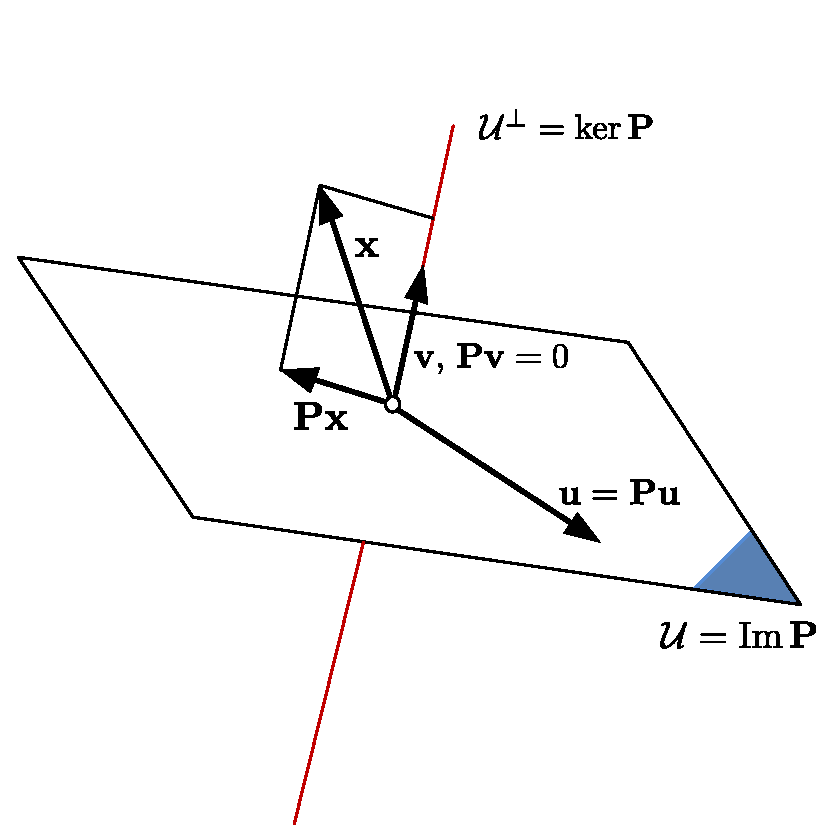
\includegraphics[width=0.7\linewidth]{fig_vl_vektory.pdf}
        \caption{ }
        \label{la:fig_vlv}
      \end{figure}
      
      Soustava rov. \ref{def_vv_homogenni} je \textbf{homogenní} a stručně ji můžeme zapsat
      \begin{equation}\label{vv_hom_zapis}
        \left(\mathbf{A} - \lambda\mathbf{I}\right) = \mathbf{0}
      \end{equation}
      Homogenní soustava má netriviální řešení, právě když je determinant matice soustavy roven nule,
      tj. v případě soustavy rov.
      \ref{def_vv_homogenni}, resp. rov. \ref{vv_hom_zapis} platí
      \begin{equation}\label{vv_hom_reseni}
        |\mathbf{A} - \lambda\mathbf{I}| = \mathbf{0}
      \end{equation}
      Determinant $A(\lambda)=|A - \lambda I|$ nazýváme \textbf{charakteristický polynom} matice $A$
      - jedná se o polynom stupně $n$ v proměnné $\lambda$, který má v oboru komplexních čísel $n$
      kořenů. Rovnici $A(\lambda)=0$ nazýváme \textbf{charakteristická rovnice matice A} - jejími
      kořeny jsou \textbf{charakteristické hodnoty} (resp. \textbf{vlastní čísla}) \textbf{matice A}.
      
      \begin{example}
        Určete spektrum matice a její spektrální poloměr následující matice
        \begin{equation*}\label{pr:spektrum_matice}
          \mathbf{A} =
          \left(
            \begin{array}{ccc}
              2  &  2    & 0 \\
             -3  & -3    & 5 \\
              0  & -0.25 & 2
            \end{array}
          \right)
        \end{equation*}
      \textbf{Řešení}: Spektrum matice je množina všech jejích vlastních čísel. Spektrální poloměr je
        maximum z absolutních hodnot vlastních čísel. Vlastní čísla určí\-me z charakteristické
        rovnice $\det(\mathbf{A}-\lambda \mathbf{I})=0$.    
        \begin{equation*}
          \textbf{A} - \lambda\textbf{I}=\left(\begin{array}{ccc}
                                                  2-\lambda  &  2          & 0 \\
                                                 -3          & -3-\lambda  & 5 \\
                                                  0          & -0.25       & 2-\lambda
                                               \end{array}
                                         \right)
        \end{equation*}
        \begin{align}
          \det(\mathbf{A}-\lambda \mathbf{I})                    &= 0           \nonumber\\
          (2-\lambda)\left(\begin{array}{cc}
                              -3-\lambda  &  5\\
                              -0.25    & 2-\lambda
                           \end{array}\right) -2\left(
                           \begin{array}{cc}
                              -3       &  5\\
                               0       & 2-\lambda
                           \end{array}\right)                   &= 0           \nonumber\\
          (2-\lambda)^2(-3-\lambda)+1.25(2-\lambda)+6(2-\lambda) &= 0           \nonumber\\
          (2-\lambda)[(2-\lambda)(-3-\lambda)+1.25+6]            &= 0           \nonumber\\
          (2-\lambda)(\lambda^2+\lambda+1.25)                    &= 0           \nonumber
        \end{align}
        \begin{equation*}
          \lambda_1 = 2, \quad\lambda_2 = -0.5+i, \quad\lambda_3=-0.5-i
        \end{equation*}
        \begin{itemize}
          \item Spektrum matice $\mathbf{A}$ je $\sigma(\mathbf{A})=\{2,-0.5+i,-0.5-i\}$.
          \item Spektrální poloměr $\rho(\mathbf{A})=\max_i|\lambda_i|=2$.
        \end{itemize}
      \end{example}
        \attachfile[icon=Paperclip, description=Matlab Determine the spectrum of a matrix 
          and its spectral radius]{../SRC/LA/matlab/LA001.m}

      %---------------------------------------------------------------
      \begin{example}
  Určete vlastní čísla a odpovídající vlastní vektory následují\-cích matic:
  \begin{displaymath}
    \mathbf{A}=\left(\begin{array}{rr}1&0.5\\3.5&4\end{array}\right), \quad
    \mathbf{B}=\left(\begin{array}{rr}3&-1 \\2.5&4\end{array}\right)
  \end{displaymath}
  \textbf{Řešení}: Vlastní čísla určíme z charakteristické rovnice: 
    $\det(\mathbf{A}-\lambda\mathbf{I})=0$. Vlastní vektory $\mathbf{x_i}$
    odpovídající vlastním číslům $\lambda_i$, jsou řešením homogenní
    soustavy rovnic $(\mathbf{A}-\lambda_i\mathbf{I})\mathbf{x_i}=0$.
    \begin{itemize}
      \item Vlastní čísla matice \textbf{A}:
        \begin{equation*}
             \textbf{A} - \lambda\textbf{I}=
               \left(\begin{array}{cc}
                        1-\lambda  &  0.5          \\
                       -3.5        &  4-\lambda
                     \end{array}
               \right)
        \end{equation*}
        \begin{align*}
           \det(\mathbf{A}-\lambda\mathbf{I}) &= 0 \\
           (1-\lambda)(4-\lambda)-\frac{7}{4} &= 0 \\
           \lambda^2-5\lambda+\frac{9}{4}     &= 0
        \end{align*}
        \begin{equation*}
           \lambda_1 = 4.5,\quad \lambda_2 = 0.5
        \end{equation*}     
    \end{itemize}

    \begin{itemize}
      \item Vlastní čísla matice \textbf{B}:
        \begin{equation*}
             \textbf{B} - \lambda\textbf{I}=
               \left(\begin{array}{cc}
                       3-\lambda  & -1             \\
                       2.5        &  4-\lambda
                     \end{array}
               \right)
        \end{equation*}
        \begin{align*}
           \det(\mathbf{B}-\lambda\mathbf{I}) &= 0 \\
           (3-\lambda)(4-\lambda)+\frac{5}{2} &= 0 \\
           \lambda^2-7\lambda+\frac{29}{2}    &= 0
        \end{align*}
        \begin{equation*}
           \lambda_1 = \frac{7+3i}{2},\quad \lambda_2 = \frac{7-3i}{2}
        \end{equation*}
    \end{itemize}
  % matice A
  Vlastní vektor matice $\mathbf{A}$ pro $\lambda_1=4.5:
  (\mathbf{A}-\lambda_1\mathbf{I})\mathbf{x_1}=0 \Rightarrow$
  \begin{align*}
    \left(
      \begin{array}{cc}
         1  -4.5  &  0.5   \\
        -3.5      &  4-4.5
      \end{array}
    \right) &\sim
    \left(
      \begin{array}{cc}
        -3.5  &  0.5       \\
        -3.5  & -0.5
      \end{array}
    \right)                         \\
    \Rightarrow\mathbf{x_1} &=
      \left(
        \begin{array}{c}
          1 \\ 7
        \end{array}
      \right)\, r, r\in\mathbb{R}, r\neq0
  \end{align*}
  Vlastní vektor matice $\mathbf{A}$ pro $\lambda_2=0.5:
  (\mathbf{A}-\lambda_1\mathbf{I})\mathbf{x_2}=0 \Rightarrow$
  \begin{align*}
    \left(
      \begin{array}{cc}
         1  -0.5  &  0.5   \\
        -3.5      &  4-0.5
      \end{array}
    \right) &\sim
    \left(
      \begin{array}{cc}
         0.5  &  0.5   \\
         3.5  &  3.5
      \end{array}
    \right)                         \\
    \Rightarrow\mathbf{x_2} &=
    \left(
      \begin{array}{c}
        -1 \\ 1
      \end{array}
    \right)\, r, r\in\mathbb{R}, r\neq0
  \end{align*}
  % matice B
  Vlastní vektor matice $\mathbf{A}$ pro $\lambda_1=\frac{7+3i}{2}:
  (\mathbf{B}-\lambda_1\mathbf{I})\mathbf{x_1}=0 \Rightarrow$
  \begin{align*}
    \left(
      \begin{array}{cc}
         3 - \frac{7+3i}{2}            &  -1                                     \\
         \frac{5}{2}                   &  4 - \frac{7+3i}{2}
      \end{array}
    \right)\sim
    \left(
      \begin{array}{cc}
        -\frac{1}{2}-\frac{3}{2}i      &  -1                                     \\
        \frac{5}{2}                    & \frac{1}{2}-\frac{3}{2}i
      \end{array}
    \right)\sim \\
    \left(
      \begin{array}{cc}
        -\frac{10}{4}                  &-\left(\frac{1}{2} -\frac{3}{2}i\right)  \\
        \frac{5}{2}                    & \frac{1}{2}-\frac{3}{2}i
      \end{array}
    \right)\sim
      \left(
        \begin{array}{cc}
          -5                           &-\left(1-3i\right)                       \\
           5                           & \left(1-3i\right)
        \end{array}
    \right)\rightarrow \\
    \mathbf{x_1}=
      \left(
        \begin{array}{c}
          -1+3i \\ 5
        \end{array}
      \right)\, r, r\in\mathbb{C}, r\neq0
  \end{align*}
  Vlastní vektor matice $\mathbf{B}$ pro $\lambda_2=\frac{7-3i}{2}:
  (\mathbf{B}-\lambda_1\mathbf{I})\mathbf{x_2}=0 \Rightarrow$
  \begin{align*}
    \left(\begin{array}{cc}
             3  - \frac{7-3i}{2}       &  -1                                     \\
            \frac{5}{2}                &  4 - \frac{7-3i}{2}
          \end{array}
    \right)\sim
    \left(\begin{array}{cc}
            -\frac{1}{2}+\frac{3}{2}i  &  -1                                     \\
            \frac{5}{2}                & \frac{1}{2}+\frac{3}{2}i
          \end{array}
    \right)\sim \\
    \left(\begin{array}{cc}
            -\frac{10}{4}              &-\left(\frac{1}{2} +\frac{3}{2}i\right)  \\
            \frac{5}{2}                & \quad\frac{1}{2}+\frac{3}{2}i
          \end{array}
    \right)\sim
      \left(\begin{array}{cc}
            -5                         &-\left(1+3i\right)                       \\
             5                         & \quad\left(1+3i\right)
          \end{array}
    \right)\rightarrow\\
    \mathbf{x_2}=
      \left(
        \begin{array}{c}
          -1-3i \\ 5
        \end{array}
      \right)\, r, r\in\mathbb{C}, r\neq0
  \end{align*}
\end{example}
%---------------------------------------------------------------
\lstinputlisting{../src/LA/img/vlastni_cisla_01.m}
\begin{lstlisting}[caption=Výpis programu pro ověření výpočtu vlastních čísel matic programem
  Matlab.]
\end{lstlisting}
%---------------------------------------------------------------
      %---------------------------------------------------------------
      \begin{example}
        Určete vlastní čísla a vlastní vektory matice
        $\mathbf{B}=\mathbf{A}^2-4\mathbf{A}+9\mathbf{A}^{-1}-\mathbf{I}$, kde $\mathbf{A}$ je matice
        $\mathbf{A}=\left(\begin{array}{cc}1&0.5\\3.5&4\end{array}\right)$.
  
        \textbf{Řešení}: (z předchozího příkladu víme, že $\lambda_1=4.5, \lambda_2=0.5$) a
         $\mathbf{I}$ jednotková matice. Označme symbolem $\lambda$ vlastní číslo matice $\mathbf{A}$
         a nechť $\mathbf{x}$ je příslušný vlastní vektor. Pak platí:
         \begin{itemize}
           \item Matice $\mathbf{A}^2$ má vlastní čísla rovna $\lambda^2$.
           \item Matice $4\mathbf{A}$ má vlastní čísla rovna $4\lambda$.
           \item Matice $9\mathbf{A}^{-1}$ má vlastní čísla rovna $\frac{9}{\lambda}$.
         \end{itemize}
         Matice $\mathbf{B}=\mathbf{A}^2-4\mathbf{A}+9\mathbf{A}^{-1}-\mathbf{I}$ má vlastní čísla ve
         tvaru  $\lambda^2-4\lambda+\frac{9}{\lambda}-1$, vlastní vektory jsou stejné jako vlastní
         vektory odpovídající vlastním číslům matice $\mathbf{A}$. Tedy:
         \begin{equation*}
             \sigma(B)=\{4.5^2-4\cdot4.5+\frac{9}{4.5}-1,\quad
             0.5^2-4\cdot0.5+\frac{9}{0.5}-1\}=\{3.25, 15.25\}
         \end{equation*}
      \end{example}
      
      \begin{definition}\label{def_rov_poly}\textbf{Rovnost dvou polynomů}:
        Řekneme, že dva polynomy \newline$f(x)=a_nx^n+a^{(n-1)}x_{(n-1)}+\ldots+a_1+a_0$ a
        $g(x)=b_mx^m+b^{(m-1)}x_{(m-1)}+\ldots+b_1+b_0$ stupňů $n$ a $m$ se sobě \textbf{rovnají}
        právě tehdy, když $m=n$ a $a_0=b_0, a_1=b_1, a_{(n-1)}=b_{(m-1)}, a_n=b_m$. V tomto případě
        také říkáme, že mnohočleny $f(x)$ a $g(x)$ jsou \textbf{totožné}.
      \end{definition}
      \begin{lemma}\label{la:eq_eqv_poly}
        Jestliže mnohočleny $f(x)$ a $g(x)$ jsou dva polynomy stupně n-tého a jestliže pro $n+1$
        různých reálných nebo komplexních čísel $x$ platí $f(x)=g(x)$, potom jsou polynomy
        \textbf{totožné}.
      \end{lemma}
  
  %============================= Kapitola: Polynomy ==========================================================
  \section{Polynomy}
    \subsection{Rozklad ryze racionální funkce na parci\-ální zlomky}
      \begin{example} 
        Rozložte na parciální zlomky lomenou racionální funkci
          $$f(x):y=\frac{7x+8}{x^2+x-2}$$
        Nejprve vypočteme nulové body jmenovatele:
          $$x^2+px+q=(x-u)(x-v)=x^2-(u+v)x+uv\rightarrow p=-(u+v),\quad q=uv$$
        Kořenové činitele  $x^2+x-2\rightarrow x_1=1, x_2=-2$ zvolíme za jmenovatele parciálních
        zlomků a rozklad hledáme ve tvaru $$\frac{7x+8}{x^2+x-2}=\frac{A}{x-1}+\frac{B}{x+2}$$
        kde $A$, $B$ jsou neznámé konstanty. Tyto konstanty určíme tak, aby rozklad platil pro každé
        $x\in\mathcal{R}-\{1,-2\}$. Po jednoduché úpravě dostaneme rovnost dvou polynomů
          $$7x+8=(A+B)x+2A-B$$
        Podle \ref{la:eq_eqv_poly} se musí rovnat koeficienty u $x$ a absolutní členy obou stran
        poslední rovnice $\Rightarrow$ dostaneme soustavu rovnic pro určení $A$ a $B$ ve tvaru:
          \begin{align}\label{la:eq_parc_example}
            % \nonumber to remove numbering (before each equation)
            7 &= A+B \\ \nonumber
            8 &= 2A+B   
          \end{align}
          $$A=5,\quad B=2 $$
        Postup, který jsme užili, nazýváme \textbf{Metodou neurčitých koeficientů}.\newline
        \emph{Pozn}: Pro určení koeficientů $A$, $B$ se užívají také jiné postupy, např. dosazování
        kořenů jmenovatele, která je výhodná zejména v případech, kdy jmenovatel lomené racionální
        funkce má jednoduché kořeny. Postupujeme tak, že rov. \ref{la:eq_parc_example}násobíme
        součinem kořenových činitelů $(x-1)(x+2)=x^2+x-2$ a dostaneme rovnici $$7x+8=A(x+2)+B(x-1)$$
        pro určení koeficientů $A$, $B$ dosazováním kořenů.
          \begin{align*}
            % \nonumber to remove numbering (before each equation)
            x=-2 &\rightarrow& -14+8=B(-2-1) \rightarrow B=2\\
            x=+1 &\rightarrow&  \,\,+7+8=A(1+2)\quad  \rightarrow A=5
          \end{align*}
      \end{example}      
  %============================= Kapitola: Vektorové prostory ================================================
  \section{Vektorové prostory se skalárním součinem}
    \subsection{Ortogonální doplňky}
      Nechť $U$ je podprostor vektorového prostoru $V$. Ortogonální doplněk $U^\bot$ obsahuje všechny
      vektory, které jsou kolmé ke každému vektoru z $U$, neboli $$\forall\vec{v}\in U^\bot\quad
      \forall\vec{u}\in U\quad \vec{u}\bot\vec{v}$$ což lze vyjádřit pomocí skalárního součinu
      $\vec{u}\cdot\vec{v} = 0$
  
      Ortogonální doplněk $U^\bot$ k podprostoru $U = \langle\vec{u}_1,\ldots,\vec{u}_k\rangle$ tedy
      hledáme jako řešení homogenní soustavy rovnic
      \begin{equation*}
        \left(
          \begin{array}{c|c}
             \vec{u}_1  &   0      \\
             \cdots     &  \vdots  \\
             \vec{u}_k  &   0
          \end{array}
        \right),
      \end{equation*}
      nuly na pravé straně při výpočtu zpravidla vynecháváme. Připomeňme také vztah
      \begin{equation}\label{LA:eq_dim_doplnek}
         \dim U + \dim U^\bot = \dim V
      \end{equation}
  
      \begin{example}\label{LA:exam_ort_doplnek01}
        Zjistěte ortogonální doplněk $$\langle(1,-3,2),(2,1,5)\rangle\bot^.$$ (Zdroj:
        \protect\cite[s.~3]{MosnaMA3}) \newline\textbf{Řešení}:
          Hledáme vektor $(x, y, z)$, jehož skalární součin je se zadanými vektory roven nule. Budeme
          tedy řešit (úpravou na Gaussův tvar pomocí elementárních úprav) homogenní soustavu rovnic
          zadanou maticí
          \begin{equation*}
             \left(
               \begin{array}{ccc|c}
                  1  &  -3  & 2 & 0 \\
                  2  &   1  & 5 & 0
               \end{array}
             \right)\sim
             \left(
               \begin{array}{ccc|c}
                  1  &  -3  & 2 & 0 \\
                  0  &   7  & 1 & 0
               \end{array}
             \right)\
          \end{equation*}
          Odtud dostáváme $$z = \alpha,\quad 7y + z = 0 \Rightarrow y = -\frac{1}{7}\alpha, \quad x
          +\frac{3}{7}\alpha + 2\alpha = 0 \Rightarrow x = -\frac{17}{7}$$ neboli $$(x, y, z) =
          \alpha\left(-\frac{17}{7}, -\frac{1}{7}, 1\right) = \alpha = (17, 1, -7).$$
  
          V dalších příkladech budeme nuly na pravé straně soustavy vynechávat a upravovat na
          výhodnější tvar
          \begin{equation*}
             \left(
               \begin{array}{ccc}
                  1  &  -3  & 2  \\
                  2  &   1  & 5
               \end{array}
             \right)\sim
             \left(
               \begin{array}{ccc}
                  1  &  -3  & 2 \\
                  0  &   7  & 1
               \end{array}
             \right)\sim
             \left(
               \begin{array}{ccc}
                  1  &   0  & \frac{17}{7}  \\
                  0  &   7  & 1
               \end{array}
             \right)\sim
             \left(
               \begin{array}{ccc}
                  7  &   0  & 17 \\
                  0  &   7  & 1
               \end{array}
             \right).
          \end{equation*}
          Odtud již snadno zjistíme, že vektor $(x, 1, -7)$ jistě vyhovuje druhé rovnici.
          Do\-sa\-dí\-me-li ho do první rovnice, dostaneme $7x + 17\cdot(-7) = 0$ a $x = 17$.
  
          Hledaný ortogonální doplněk je tedy lineární obal $$\langle(17, 1, -7)\rangle^\bot.$$
          \begin{figure}[ht!]
            \centering
            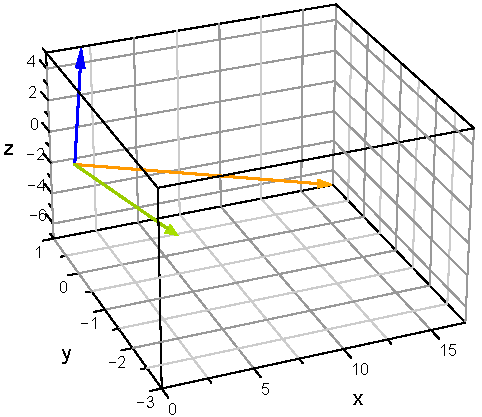
\includegraphics[width=0.8\linewidth]{ort_doplnek_exam01.pdf}
            \caption[Ortogonální doplněk]{Vizualizace vektorového prostoru a jeho ortogonálního
                     doplňku pomocí sw MatLab - MuPAD příkazem:\newline
                     \texttt{plot(plot::Arrow3d([1,-3,2]),plot::Arrow3d([2,1,5]), 
                     plot::Arrow3d([17,1,-7]))}}
            \label{LA:fig_ort01}
          \end{figure}
      \end{example}
  
      Výsledek předchozího příkladu \ref{LA:exam_ort_doplnek01} lze interpretovat tak, že jsme našli všechny 
      vektory, které jsou kolmé na rovinu určenou vektory ze zadání. Rovina je útvar dvojrozměrný a protože 
      prostor všech vektorů je trojrozměrný, musí nutně mít podprostor ortogonálních vektorů ve shodě se 
      vztahem \ref{LA:eq_dim_doplnek} pouze jednu dimenzi. Vše je dobře patrné z obr. \ref{LA:fig_ort01}
  
    \section{Vektory}
  %---Formulář operace s vektory----------- 
   \vskip5mm\hrule
  \emph{Zadejte složky vektoru} $\vec{a}:$
    \vskip2mm
    \hskip8mm$\vec{a}$   =  
      \TextField[width=15mm,name=Inputv1.First,borderstyle=I,value={},align=1,
                validate={v1x=this.getField("Inputv1.First");}]{ }{\ $\vec{x}\ +$}
      \TextField[width=15mm,name=Inputv1.Second,borderstyle=I,value={},align=1,
                validate={v1y=this.getField("Inputv1.Second");}]{ }{\ $\vec{y}\ +$}  
      \TextField[width=15mm,name=Inputv1.Third,borderstyle=I,value={},align=1,
                validate={v1z=this.getField("Inputv1.Third");}]{ }{\ $\vec{z}$}
    \vskip2mm
      \emph{a vektoru} $\vec{b}$:
    \vskip2mm
    \hskip8mm$\vec{b}$ = 
      \TextField[width=15mm,name=Inputv2.First,borderstyle=I,value={},align=1,
                validate={v2x=this.getField("Inputv2.First");}]{ }{\ $\vec{x}\ +$}  
      \TextField[width=15mm,name=Inputv2.Second,borderstyle=I,value={},align=1,
                validate={v2y=this.getField("Inputv2.Second");}]{ }{\ $\vec{y}\ +$} 
      \TextField[width=15mm,name=Inputv2.Third,borderstyle=I,value={},align=1,
                validate={v2z=this.getField("Inputv2.Third");}]{ }{\ $\vec{z}$}  
    \vskip2mm\hrule\vskip4mm 
    \emph{Operace s vektory:} % \centering vystředí jediný řádek textu:
                                         % \centering{text}
    \vskip2mm
    % Vektorový součet
    \PushButton[name=pb1,borderstyle=B,borderwidth=1.5,onclick={vecsum();}]
       {\hskip2mm$\vec{a}+\vec{b}$\hskip2mm} =   
          \TextField[width=15mm,name=Output.First,borderstyle=I,value={},align=1,
                    validate={output1=this.getField("Output.First");}]{ }{\ $\vec{x}\ +$} 
          \TextField[width=15mm,name=Output.Second,borderstyle=I,value={},align=1,
                    validate={output2=this.getField("Output.Second");}]{ }{\ $\vec{y}\ +$} 
          \TextField[width=15mm,name=Output.Third,borderstyle=I,value={},align=1,
                    validate={output3=this.getField("Output.Third");}]{ }{\ $\vec{z}$}
    \vskip2mm
    % skalární součin
    \PushButton[name=pb2,borderstyle=B,borderwidth=1.5,onclick={innerpro();}]
       {\hskip2mm$\vec{a}\cdot\vec{b}$\hskip2mm} = 
          \TextField[width=20mm,name=Output.Fourth,borderstyle=I,value={0},
                    align=1,validate={output4=this.getField("Output.Fourth");},
                    calculate={output4.value}]{ }
    \vskip2mm
    \PushButton[name=pb3,borderstyle=B,borderwidth=1.5,onclick={}]
       {\hskip2mm$\theta$\hskip2mm} = 
          \TextField[width=20mm,name=Output.Fifth,borderstyle=I,value={0},
                    align=1,validate={output5=this.getField("Output.Fifth");}]{ }\hskip2mm$^\circ$
    \vskip2mm                  
    % vektorový součin
    \PushButton[name=pb4,borderstyle=B,borderwidth=1.5,onclick={outerpro();}]
       {\hskip2mm$\vec{a}\times\vec{b}$\hskip2mm} = 
          \TextField[width=15mm,name=Output.Sixth,borderstyle=I,value={0},
                     align=1,validate={output6=this.getField("Output.Fifth");},
                     calculate={output1.value}]{ }{\ $\vec{x}\ +$}
          \TextField[width=15mm,name=Output.Seventh,borderstyle=I,value={0},
                     align=1,validate={output7=this.getField("Output.Sixth");},
                     calculate={output1.value}]{ }{\ $\vec{y}\ +$}
          \TextField[width=15mm,name=Output.Eighth,borderstyle=I,value={0},
                     align=1,validate={output8=this.getField("Output.Eighth");},
                     calculate={output1.value}]{ }{\ $\vec{z}$} 
  \vskip5mm\hrule
  %----------------------------------------
  
\printbibliography[title={Seznam literatury}, heading=subbibliography]
\addcontentsline{toc}{section}{Seznam literatury}  
     
%----------------------------------------------------------------------------------------------------